\documentclass{report}


\usepackage[T1]{fontenc}
\usepackage[utf8]{inputenc}
\usepackage{amsmath}


\usepackage{multirow}

\usepackage{enumerate}
\usepackage{trfsigns}
\usepackage{graphicx}
\usepackage{fancyhdr}
\usepackage{lettrine}
\usepackage{hyperref}
\usepackage{subcaption}
\usepackage{tikz}
\usepackage{cite}
\usepackage{listings}
\usepackage[nottoc, numbib]{tocbibind}
\usepackage[ngerman]{babel}
\usepackage[Glenn]{fncychap}
\usepackage{trfsigns}
\usepackage{parskip}
\usepackage{microtype}


\usetikzlibrary{shapes}
\usetikzlibrary{arrows}
\usetikzlibrary{arrows.meta,topaths}
\usetikzlibrary{bending}
\usetikzlibrary{calc}
\title{Elektrotechnik 1 Praktikum 1}


\usepackage[
	includehead,
	headheight = 17mm,
	footskip = \dimexpr\headsep+\ht\strutbox\relax,
	tmargin = 0mm,
	bmargin = \dimexpr17mm+2\ht\strutbox\relax,
]{geometry}

\usepackage{anyfontsize}
\usepackage{float}
\usepackage{xcolor}

\definecolor{DarkGreenBlue}{HTML}{264653}
\definecolor{LightGreenBlue}{HTML}{2A9D8F}
\definecolor{LightOrange}{HTML}{E9C46A}
\definecolor{DarkOrange}{HTML}{F4A261}
\definecolor{RedOrange}{HTML}{E76F51}
\definecolor{BrightRed}{HTML}{D62828}
\definecolor{DeepBlue}{HTML}{003049}

\lstdefinestyle{code}{
	backgroundcolor=\color{backcolour},
	commentstyle=\color{codegreen},
	keywordstyle=\color{magenta},
	numberstyle=\tiny\color{codegray},
	stringstyle=\color{codepurple},
	basicstyle=\ttfamily\footnotesize,
	breakatwhitespace=false,
	breaklines=true,
	captionpos=b,
	keepspaces=true,
	numbers=left,
	numbersep=5pt,
	showspaces=false,
	showstringspaces=false,
	showtabs=false,
	tabsize=2
}

\definecolor{codegreen}{rgb}{0,0.6,0}
\definecolor{codegray}{rgb}{0.5,0.5,0.5}
\definecolor{codepurple}{rgb}{0.502,0.502,0.0}
\definecolor{backcolour}{rgb}{0.95,0.95,0.95}

\pagestyle{fancy}
\fancyhead[L]{\leftmark}
\fancyhead[R]{}
\fancyfoot[L]{}
\fancyfoot[C]{\thepage}
\fancyfoot[R]{\includegraphics[scale=0.2]{../assets/images/haw.jpg}}
\renewcommand\headrulewidth{0.5pt}


\begin{document}


\thispagestyle{empty}
\begin{tikzpicture}[overlay,remember picture]
	\thispagestyle{empty}
	\fill[black!2] (current page.south west) rectangle (current page.north east);

	\begin{scope}[transform canvas ={rotate around ={45:($(current page.north west)+(-.5,-6)$)}}]

		\shade[rounded corners=18pt, left color=DarkGreenBlue, right color=LightGreenBlue] ($(current page.north west)+(-.5,-6)$) rectangle ++(9,1.5);

	\end{scope}

	\begin{scope}[transform canvas ={rotate around ={45:($(current page.north west)+(.5,-10)$)}}]

		\shade[rounded corners=18pt, left color=LightOrange,right color=DarkOrange] ($(current page.north west)+(0.5,-10)$) rectangle ++(15,1.5);

	\end{scope}

	\begin{scope}[transform canvas ={rotate around ={45:($(current page.north west)+(0.5,-10)$)}}]

		\shade[rounded corners=8pt, right color=DarkOrange, left color=LightOrange] ($(current page.north west)+(1.5,-9.55)$) rectangle ++(7,.6);

	\end{scope}

	\begin{scope}[transform canvas ={rotate around ={45:($(current page.north)+(-1.5,-3)$)}}]

		\shade[rounded corners=12pt, left color=DeepBlue!80, right color=DeepBlue!60] ($(current page.north)+(-1.5,-3)$) rectangle ++(9,0.8);

	\end{scope}

	\begin{scope}[transform canvas ={rotate around ={45:($(current page.north)+(-3,-8)$)}}]

		\shade[rounded corners=28pt, left color=BrightRed, right color=BrightRed!80] ($(current page.north)+(-3,-8)$) rectangle ++(15,1.8);

	\end{scope}

	\begin{scope}[transform canvas ={rotate around ={45:($(current page.north west)+(4,-15.5)$)}}]

		\shade[rounded corners=25pt, left color=RedOrange, right color=DarkOrange] ($(current page.north west)+(4,-15.5)$) rectangle ++(30,1.8);

	\end{scope}

	\begin{scope}[transform canvas ={rotate around ={45:($(current page.north west)+(13,-10)$)}},]

		\shade[rounded corners=22pt, left color=DeepBlue,right color=DarkGreenBlue] ($(current page.north west)+(13,-10)$) rectangle ++(15,1.5);

	\end{scope}

	\begin{scope}[transform canvas ={rotate around ={45:($(current page.north west)+(18,-8)$)}},]

		\shade[rounded corners=8pt, left color=DarkOrange] ($(current page.north west)+(18,-8)$) rectangle ++(15,0.6);

	\end{scope}

	\begin{scope}[transform canvas ={rotate around ={45:($(current page.north west)+(19,-5.65)$)}},]

		\shade[rounded corners=12pt, left color=RedOrange] ($(current page.north west)+(19,-5.65)$) rectangle ++(15,0.8);

	\end{scope}

	\begin{scope}[transform canvas ={rotate around ={45:($(current page.north west)+(20,-9)$)}}]

		\shade[rounded corners=20pt, left color=BrightRed, right color=BrightRed!80] ($(current page.north west)+(20,-9)$) rectangle ++(14,1.2);

	\end{scope}

	\draw[ultra thick,gray] ($(current page.center)+(5,2)$) -- ++(0,-3cm) node[midway,left=0.25cm,text width=5cm,align=right,black!75]{{\fontsize{25}{30} \selectfont 
\includegraphics[width=\textwidth]{./assets/img/HAW_logo.png}}} node[midway,right=0.25cm,text width=6cm,align=left,orange]{{\fontsize{70}{86} \selectfont 2023}};

	\node at ($(current page.center)+(0,-4)$) {{\fontsize{40}{72} \selectfont Leistungselektronik}};

	\node[text width=8cm,align=center] at ($(current page.center)+(0,-6.5)$) {{\fontsize{16}{20} \selectfont \textcolor{orange}{ \bf \today}} \\[3pt] Fynn Beck\\[3pt] PF: Emily Antosch 2519935 \\[3pt] Lara Böhme\\[3pt]};

\end{tikzpicture}

\newpage

\tableofcontents

\listoffigures

\newpage

\listoftables

\newpage

\chapter{Regenerative Energien - Windkraftanlage}
\section{Einleitung}

In diesem Praktikum wird eine Windkraftanlage anhand ihrer Eigenschaften untersucht. Dabei wird insbesondere der Anschluss der Ansynchronmaschine, die in dieser Anlage als Generator dient, an das Versorgungsnetz betrachtet.

\section{Kenndaten der Windkraftanlage}

Die folgenden Daten wurden dem Typenschild der Windkraftanlage entnommen:

\begin{itemize}
	\item Nennleistung: $P_{N} = 5kW$
  \item Nennspannung: $U_{N} = 400V$
		\item Verdrahtungsart: Dreieck
	\item Nenndrehzahl des Rotors: $n_{N} = 1450min^{-1}$
	\item Polpaarzahl: $p = 2$
	\item Läufernennspannung: $U_{NL} = Y500V$
		\item Läufernennstrom: $I_{NL} = 6,2A$
\end{itemize}

\section{Drehzahl-Drehmoment-Kennlinie der Windkraftanlage}

Im ersten Teil der Versuchsreihe wird die Drehzahl-Drehmoment-Kennlinie der Windkraftanlage ermittelt. Dazu wird die Windkraftanlage mit einem Gleichstrommotor verbunden, der die Windkraftanlage mit einer variablen Drehzahl versorgt. Die Drehzahl-Drehmoment-Kennlinie wird dann durch Messung der Drehzahl und des Drehmoments bei verschiedenen Windgeschwindigkeiten ermittelt. Alle Messungen, die zu einer Windgeschwindigkeit gehören, werden in einem Graphen und alle Graphen werden in einem Diagramm zusammengefasst (siehe dazu Abbildung \ref{fig:zahl_moment}). Der genaue Aufbau für diesen Versuchsteil ist in Abbildung \ref{fig:asm_aufbau_umrichter} dargestellt.

Dazu soll zunächst das Nenndrehmoment berechnet werden:

\begin{equation}
  \label{eq:1}
  M_{i} = \frac{P}{2\pi\cdot n_{N}\cdot \frac{1}{60s}} = \frac{5kW}{2\pi \cdot 1450min^{-1} \cdot \frac{1}{60s}} = 32,93Nm
\end{equation}



\begin{table}[]
\begin{tabular}{|c|c|c|}
Windgeschwindigkeit & Drehzahl & Drehmoment \\ \hline
\multirow{11}{*}{5} & 650      & 5,9        \\ \cline{2-4}
                    & 750      & 5,8        \\ \cline{2-4}
                    & 850      & 5,4        \\ \cline{2-4}
                    & 950      & 4,3        \\ \cline{2-4}
                    & 1050     & 3,1        \\  \cline{2-4}
                    & 1150     & 2,2        \\ \cline{2-4}
                    & 1250     & 1,2        \\ \cline{2-4}
                    & 1350     & 0,95       \\ \cline{2-4}
                    & 1450     & 1          \\ \cline{2-4}
                    & 1550     & 1          \\ \cline{2-4}
                    & 1650     & 1 \\ \hline
\multirow{11}{*}{9} & 650      & 6,5        \\ \cline{2-4}
                    & 750      & 9,3        \\ \cline{2-4}
                    & 850      & 12,7       \\ \cline{2-4}
                    & 950      & 14,5       \\ \cline{2-4}
                    & 1050     & 16         \\ \cline{2-4}
                    & 1150     & 17,4       \\ \cline{2-4}
                    & 1250     & 17,5       \\ \cline{2-4}
                    & 1350     & 17         \\ \cline{2-4}
                    & 1450     & 16,5       \\ \cline{2-4}
                    & 1550     & 15         \\ \cline{2-4}
                    & 1650     & 14 \\ \hline
\multirow{11}{*}{13} & 650      & 2          \\ \cline{2-4}
                     & 750      & 4,6        \\ \cline{2-4}
                     & 850      & 8,6        \\ \cline{2-4}
                     & 950      & 12,5       \\ \cline{2-4}
                     & 1050     & 17         \\ \cline{2-4}
                     & 1150     & 21         \\ \cline{2-4}
                     & 1250     & 24         \\ \cline{2-4}
                     & 1350     & 26         \\ \cline{2-4}
                     & 1450     & 28         \\ \cline{2-4}
                     & 1550     & 29         \\ \cline{2-4}
                     & 1650     & 30 \\ \hline
\multirow{11}{*}{17} & 650      & 1          \\ \cline{2-4}
                     & 750      & 1,5        \\ \cline{2-4}
                     & 850      & 3,4        \\ \cline{2-4}
                     & 950      & 7          \\ \cline{2-4}
                     & 1050     & 11,5       \\ \cline{2-4}
                     & 1150     & 16         \\ \cline{2-4}
                     & 1250     & 20         \\ \cline{2-4}
                     & 1350     & 25         \\ \cline{2-4}
                     & 1450     & 28         \\ \cline{2-4}
                     & 1550     & 30         \\ \cline{2-4}
                     & 1650     & 31 		\\\hline
\end{tabular}
\caption{Tabelle der Messwerte für die Drehzahl-Drehmoment-Kennlinien im Bereich $650min^{-1}...1650min^{-1}$}
\label{tab:drehzahl_drehmoment}
\end{table}

% FIXME: Bild fehlt
\begin{figure}[!ht]
	\centering
	\includegraphics[width=0.8\textwidth]{./assets/images/zahl_moment.png}
	\caption{Drehzahl-Drehmoment-Kennlinien der Windkraftanlage}
	\label{fig:zahl_moment}
\end{figure}

\section{Drehzahl-Leistungs-Kennlinie der Windkraftanlage}

Im zweiten Teil der Versuchsreihe wird die Drehzahl-Leistungs-Kennlinie der Windkraftanlage ermittelt. Dazu werden die Messungen aus dem vorherigen Versuch analysiert und zu jeder Kennlinie wird eine entsprechende Drehzahl-Leistungskennlinie erzeugt. Alle Ergebnisse, die zu einer Windgeschwindigkeit gehören, werden in einem Graphen und alle Graphen werden in einem Diagramm zusammengefasst (siehe dazu Abbildung \ref{fig:zahl_leistung}).

% FIXME: Bild fehlt
\begin{figure}[!ht]
	\centering
	\includegraphics[width=0.8\textwidth]{./assets/images/zahl_leistung.png}
	\caption{Drehzahl-Leistungs-Kennlinien der Windkraftanlage}
	\label{fig:zahl_leistung}
\end{figure}

\section{Windkraftanlage mit direkter Netzkopplung}

\subsection{Stationäres Verhalten}

In diesem Teil des Labor wird das stationäre Verhalten, also das Verhalten bei konstanter Windgeschwindigkeit, der Windkraftanlage mit direkter Netzkopplung untersucht. Dazu wird die Windkraftanlage mit einem Gleichstrommotor verbunden, der die Windkraftanlage mit einer konstanten Drehzahl versorgt. Da es sich hier um eine direkte Kopplung mit dem Netz handelt, wird zusätzlich eine Blindleistungskompensationsanlage eingebaut, die einen Teil der Blindleistung kompensiert. Eine Steuerung von diesem Prozess ist also nur indirekt möglich.

\begin{figure}[!ht]
	\centering
	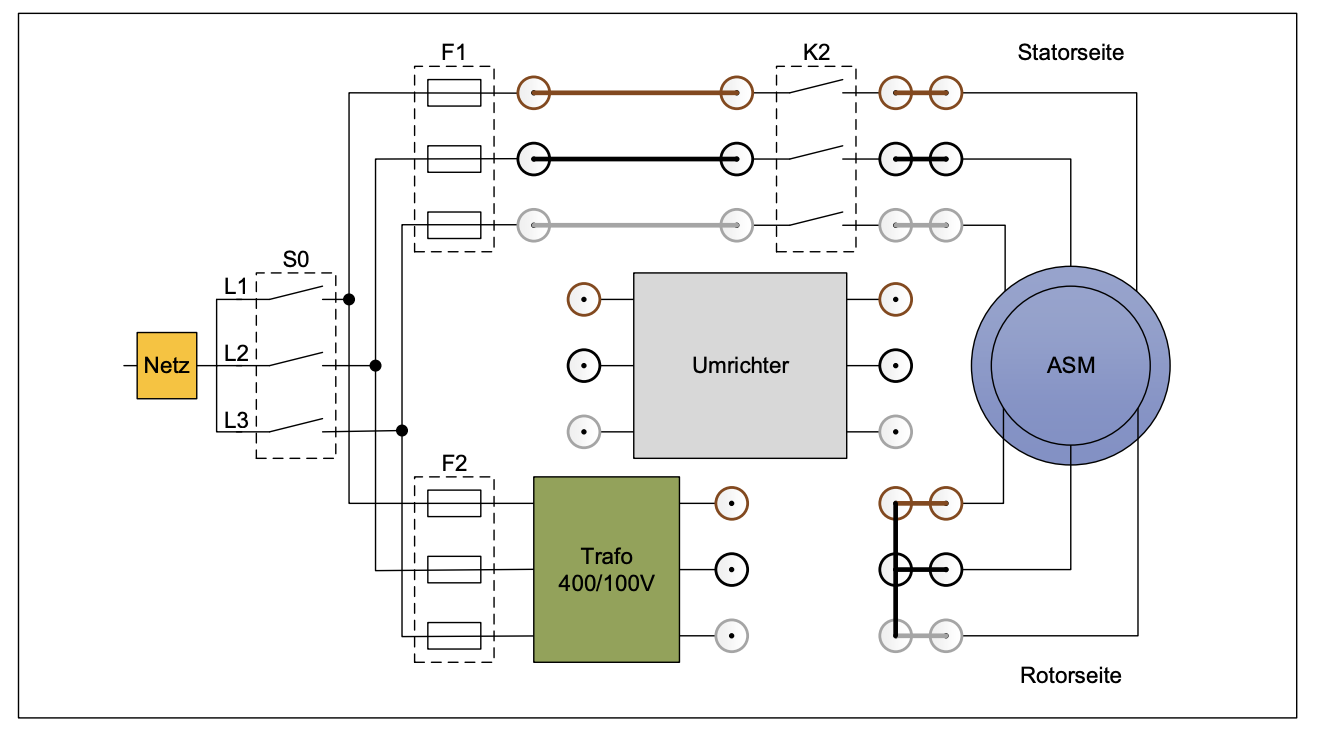
\includegraphics[width=0.8\textwidth]{./assets/images/asm_aufbau_direkt.png}
	\caption{Leistung der Windkraftanlage als Funktion der Windgeschwindigkeit}
	\label{fig:aufbau_direkt}
\end{figure}

Es wird die abgegebene Leistung $P_{el}$ als Funktion der Windgeschwindigkeit $v_{\mathrm{wind}}$ gemessen. Außerdem soll das Wertetripel $(n, M, \theta)$ notiert werden. Die Ergebnisse dieser Messung im Verhältnis zur Windgeschwindigkeit $v_{\mathrm{wing}}$ im Bereich $4m/s\leq v_{\mathrm{wind}} \leq 17m/s$ finden sich in Tabelle~\ref{tab:direkt_pel}.
\begin{table}[!ht]
\begin{tabular}{|c|c|c|c|c|}
Windgeschwindigkeit & elektrische Leistung & Drehzahl & Drehmoment & Pitchwinkel \\
  \midrule
4                   & -840                 & 1498     & -1,5       & 0           \\
5                   & -750                 & 1498     & -1,5       & 0           \\
6                   & -660                 & 1498     & -0,55      & 0           \\
7                   & 20                   & 1503     & 3,5        & 0           \\
8                   & 800                  & 1510     & 8,5        & 0           \\
9                   & 1550                 & 1515     & 13,5       & 0           \\
10                  & 2300                 & 1520     & 19,5       & 0           \\
11                  & 3100                 & 1526     & 23         & 0           \\
12                  & 3600                 & 1530     & 26,5       & 0           \\
13                  & 4050                 & 1530     & 29         & 0           \\
14                  & 4200                 & 1525     & 30         & 1           \\
15                  & 4200                 & 1535     & 30         & 2           \\
16                  & 4200                 & 1535     & 30         & 2           \\
17                  & 4200                 & 1535     & 30         & 2
\bottomrule
\end{tabular}
\caption{Die Messwerte für die ASM mit direkter Netzkopplung, ohne Blindleistungskompensationsanlage und bei ruhigem Windgang}
\label{tab:asm_direkt_ohneBlind_ruhig}
\end{table}
Aus der Tabelle lässt sich nun der Wirkungsgrad der Maschine berechnen. Wir rechnen dafür:

\begin{equation}
  \label{eq:3}
  P_{mech} = M_{i} \cdot n_{N} \cdot \frac{1}{60s} \cdot 2\pi
\end{equation}
die mechanische Leistung für einen Betriebspunkt $v_{\mathrm{wind}}$ aus. Im Anschluss kann für diesen Betriebspunkt dann auch der Wirkungsgrad berechnet werden.

\begin{equation}
  \label{eq:2}
  \eta = \frac{P_{el}}{P_{mech}}
\end{equation}
Bei der Windgeschwindigkeit $v_{\mathrm{wind}} = 11 \frac{m}{s}$ wird nun mit dem Oszilloskop die Netz-Sternspannung $u_{2N}(t)$ und der zugehörige Netz-Leiterstrom $i_{2}(t)$ gemessen. Darüber hinaus soll auch der Ständerstrom $i_{S2}(t)$ und der Rotorstrom $u_{R2}(t)$ aufgezeichnet werden. Die Messung wird in Abbildung \ref{fig:netz} dargestellt.

\begin{figure}[!ht]
	\centering
	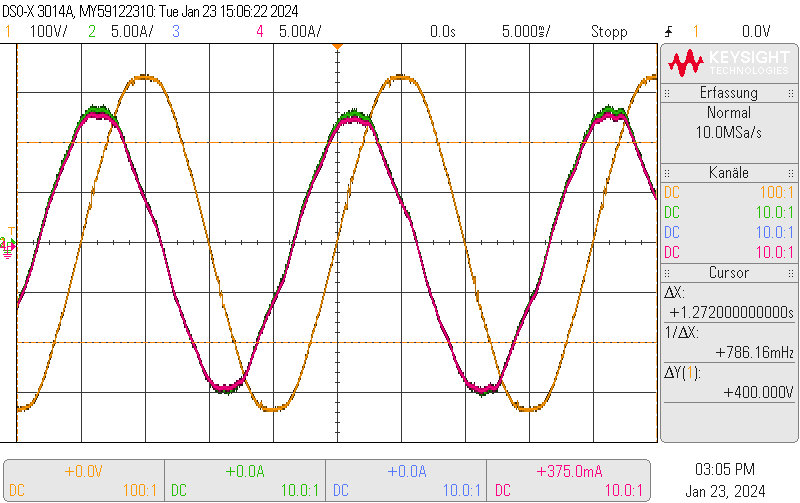
\includegraphics[width=0.8\textwidth]{./assets/images/3_3_1_ohneRotorstrom.png}
	\caption{Messung der Netz-Sternspannung $u_{2N}(t)$ und des Netz-Leiterstroms $i_{2}(t)$ bei $v_{\mathrm{wind}} = 11 \frac{m}{s}$}
	\label{fig:oszi_direkt_spannung}
\end{figure}

\begin{figure}[!ht]
	\centering
	\includegraphics[width=0.8\textwidth]{./assets/images/3_3_2_ohneRotorstrom.png}
	\caption{Messung der Netz-Sternspannung $u_{2N}(t)$ und des Netz-Leiterstroms $i_{2}(t)$ bei $v_{\mathrm{wind}} = 11 \frac{m}{s}$ und Blindleistungskompensation}
	\label{fig:oszi_direkt_spannung_mitKomp}
\end{figure}

Die Blindleistungskompensation in~\ref{fig:oszi_direkt_spannung_mitKomp} verschiebt den Strom weiter in Phase mit der Spannung. Allerdings schwingen die Kondensatoren mit den Induktivitäten des Netzes und erzeugen so Oberschwingungen. Die Blindleistungskompensation ist also nicht ideal.


\subsection{Dynamisches Verhalten}

Bei dem dynamischen Verhalten der Windkraftanlage wird die Windkraftanlage wieder über die Gleichstrommaschine betrieben. Dabei wird die Voreinstellung allerdings auf \textit{turbulent} gestellt und der Einfluss einer Windböe auf die Leistung der Windkraftanlage wird untersucht.


Insbesondere soll hier der Leistungsfluss innerhalb der Windkraftanlage, die eingespeiste Leistung und die Drehzahl betrachtet werden.

Im turbulenten Modus schwankt die eingespeiste Wirkleistung, die die Windkraftanlage in das Netzeinspeist, in Abhängigkeit von $z_{0}$ also der Oberflächenbeschaffenheit der Umgebung, stark. Proportional zu der Schwankung der Wirkleistung schwankt auch der Ist-Wert der Drehzahl stärker als bei ruhigem Windgang, jedoch deutlich leichter. Auf dem Oszilloskopbild ist auch eine Änderung der Scheitelwerte der Ströme zu erkennen. Allerdings nimmt die ASM immer noch induktive Blindleistung auf und diese bleibt auch weiterhin ziemlich stabil. Am Leistungsfluss innerhalb der ASM ändert sich auch bei turbulenten Windverhältnissen wenig.

Im Anschluss wird die Leistung, die von der Windkraftanlage ins Netz gespeist wird, auf $1500$W begrenzt. Durch die Begrenzung der Wirkleistung, die maximal ins Netz eingespeist werden darf, wird die Drehzahl der ASM abgesenkt. Der Leistungsbeiwert $c_{p}$ verlässt die optimale Betriebskurve und der Pitchwinkel $\Theta$ steigt stark an. Dieser schwankt auch, in Abhängigkeit von der Windgeschwindigkeit, und begrenzt damit die Wirkleistung. Eine solche Maßnahme kann sinnvoll sein, damit der Betreiber der WEA kontrollieren kann, nicht zu viel Leistung ins Netz einzuspeisen, auch wenn die Windgeschwindigkeit schwankt.


Es werden nun erneut die Netz-Sternspannung $u_{2N}(t)$, der Netz-Leiterstrom $i_{2}(t)$, der Ständerstrom $i_{S2}(t)$ und der Rotorstrom $u_{R2}(t)$ gemessen. Die Messungen sind in Abbildung~\ref{fig:oszi_direkt_dynamisch}

\begin{figure}[!ht]
	\centering
	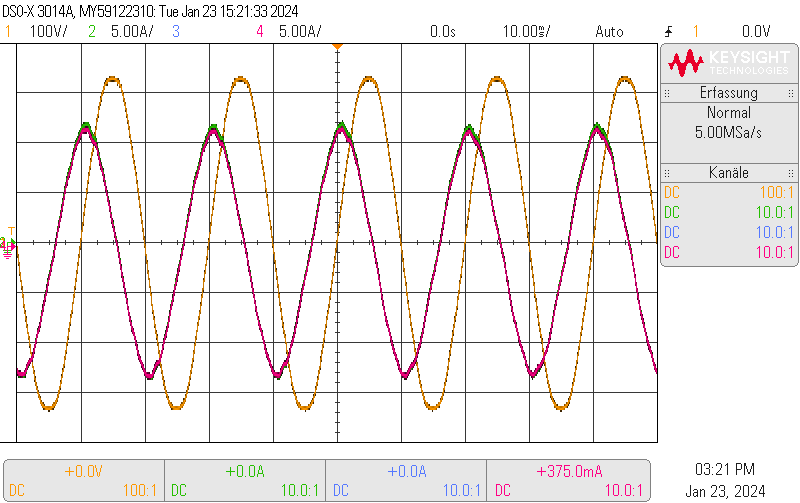
\includegraphics[width=0.8\textwidth]{./assets/images/3_3_3_ohneRotorstrom.png}
	\caption{Messung der Netz-Sternspannung $u_{2N}(t)$ und des Netz-Leiterstroms $i_{2}(t)$ bei $v_{\mathrm{wind}} = 11 \frac{m}{s}$}
	\label{fig:oszi_direkt_dynamisch}
\end{figure}

\section{Windkraftanlage mit Vollumrichter}

\subsection{Stationäres Verhalten}
\label{subsec:stat-voll}

Im nächsten Teil der Versuchsreihe wird die Windkraftanlage mit einem Vollumrichter betrieben. Dazu wird die Anlage wie in Abbildung \ref{fig:umrichter_aufbau} verschaltet.


\begin{figure}[!ht]
  \centering
  \includegraphics[width=0.8]{./assets/img/asm_aufbau_umrichter.png}
  \caption{Aufbau der Windkraftanlage mit Umrichter}
  \label{fig:aufbau_umrichter}
\end{figure}

Wie im vorherigen Versuch wird auch hier die Leistung der Windkraftanlage als Funktion der Windgeschwindigkeit $v_{\mathrm{wind}}$ gemessen. Auch hier soll das Wertetripel $(n, M, \theta)$ wieder mitaufgezeichnet werden. Die Messungen sind in Tabelle~\ref{tab:umrichter_pel} dargestellt.

\begin{table}[!ht]
\begin{tabular}{|c|c|c|c|c|}
Windgeschwindigkeit & elektrische Leistung & Drehzahl & Drehmoment & Pitchwinkel \\
4                   & 5                   & 800      & 5,5        & 0           \\
5                   & 15                   & 800      & 5,5        & 0           \\
6                   & 30                   & 830      & 6,3        & 0           \\
7                   & 550                  & 1102     & 9,9        & 0           \\
8                   & 1050                 & 1260     & 12,5       & 0           \\
9                   & 1750                 & 1425     & 16         & 0           \\
10                  & 2450                 & 1530     & 20         & 0           \\
11                  & 3000                 & 1570     & 24,5       & 0           \\
12                  & 3650                 & 1610     & 28         & 0           \\
13                  & 4200                 & 1650     & 30         & 0           \\
14                  & 4200                 & 1650     & 30         & 2           \\
15                  & 4200                 & 1535     & 30         & 4           \\
16                  & 4200                 & 1535     & 30         & 5           \\
17                  & 4200                 & 1535     & 30         & 6
\end{tabular}
\end{table}
Es lässt sich erkennen, dass die ersten Windgeschwindigkeit, bei der mit Sicherheit Leistung ins Netz eingespeist wird, bei $v_{\mathrm{wind}} = 6m/s$ liegt.
Wie im ersten Teil des Versuchs soll nun die Netz-Sternspannung $u_{2N}(t)$ und der Netz-Leiterstrom $i_{2}(t)$ bei einer Windgeschwindigkeit von $v_{\mathrm{wind}} = 11 \frac{m}{s}$ gemessen werden. Die Messung ist in Abbildung~\ref{fig:oszi_umrichter} dargestellt.

\begin{figure}[!ht]
  \centering
  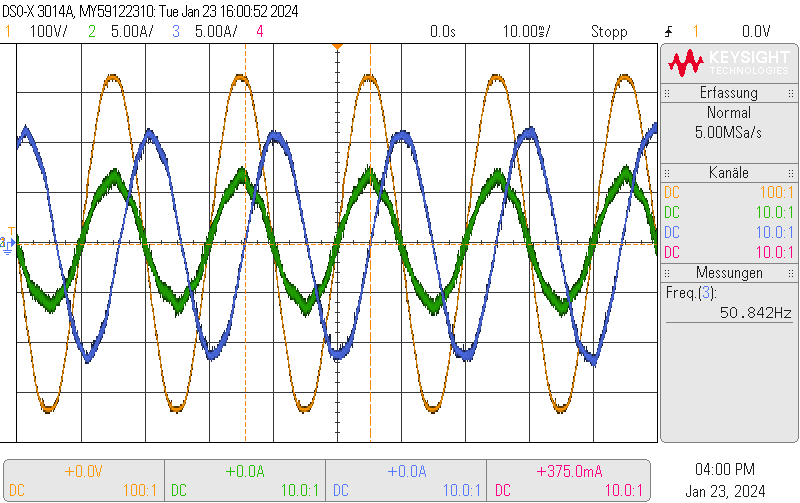
\includegraphics[width=0.8\textwidth]{./assets/images/3_4_1_ohneRotorstrom.png}
  \caption{Die Netz-Sternspannung und Netz-Leiterstrom bei einer Windgeschwindigkeit von 11m/s}
  \label{fig:oszi_umrichter}
\end{figure}

\subsection{Dynamisches Verhalten}

Die Anlage wird wieder im turbulenten Modus betrieben. Das Verhalten der ASM im Vergleich zur direkten Netzkopplung ist deutlich an der eingespeisten Wirkleistung zu erkennen. Diese schwankt deutlich weniger als bei der direkten Netzkopplung. Die Drehzahl der ASM schwankt auch deutlich weniger als bei der direkten Netzkopplung. Im Betriebspunkt bei $v_{\mathrm{wind}} = 11m/s$ hat der Arbeitspunkt die optimale $c_{p}$-$\lambda$-Kennlinie noch nicht verlassen. Eine ASM mit Vollumrichter ist daher deutlich besser dafür geeignet, Leistung ins Netz einzuspeisen, auch bei turbulenten Windverhältnissen als eine ASM, die direkt mit dem Netz gekoppelt ist.

\begin{figure}[!ht]
  \centering
  \includegraphics[width=0.8\textwidth]{./assets/images/3_4_2_ohneRotorstrom.png}
  \caption{Die Netz-Sternspannung und Netz-Leiterstrom bei einer Windgeschwindigkeit von 11m/s und turbulenter Windgeschwindigkeit}
  \label{fig:oszi_umrichter_turbulent}
\end{figure}

Wird die Wirkleistung wieder auf $1500W$ begrenzt, so verlässt der Arbeitspunkt erneut die optimale $c_{p}$-$\lambda$-Kennlinie. Der Pitchwinkel steigt an und deckelt so die einzuspeisende Wirkleistung bei gegebener Windgeschwindigkeit.

Über die direkte Regelung der Netzblindleistung, kann eine Verschiebung des Stromes zur Spannung wahrgenommen werden. Die Verschiebungsblindleistung $Q_{1}$ wird durch den Vollumrichter gesteuert. Dadurch ermöglicht dieser Aufbau, im Gegensatz zur direkten Netzkopplung, eine direkte Steuerung der Blindleistung. Die aufgenommene Blindleistung der WEA ist also vollkommen unabhängig von der Windgeschwindigkeit oder der Drehzahl.

\section{Windkraftanlage mit doppelter Einspeisung}
\label{sec:windkr-mit-dopp}

Im letzten Teil der Versuchsreihe wird die Windkraftanlage mit doppelter Einspeisung betrieben. Dazu wird die Anlage wie in Abbildung \ref{fig:aufbau_dopp} verschaltet. Wie im vorherigen Versuch wird auch hier die Leistung der Windkraftanlage als Funktion der Windgeschwindigkeit $v_{\mathrm{wind}}$ gemessen. Die Messung wird in Abbildung \ref{fig:leistung_dopp} dargestellt.

\begin{figure}[!ht]
  \centering
  \includegraphics[width=0.8\textwidth]{./assets/images/asm_aufbau_doppelt.png}
  \caption{Der Aufbau der doppelt eingespeisten ASM}
  \label{fig:asm_aufbau_doppelt}
\end{figure}


\begin{table}[!ht]
\begin{tabular}{|c|c|c|c|c|c|c|}
Windgeschwindigkeit & elektrische Leistung & Drehzahl & Drehmoment & Pitchwinkel & Statorleistung & Rotorleistung   1   2 \\

4                   & 10                   & 1045     & 6          & 0           & 400            & -270          \\
5                   & 25                   & 1050     & 6,16       & 0           & 400            & -280          \\
6                   & 50                   & 1053     & 6,16       & 0           & 400            & -285          \\
7                   & 400                  & 1135     & 8,9        & 0           & 840            & -330          \\
8                   & 950                  & 1290     & 11,9       & 0           & 1250           & -250          \\
9                   & 1620                 & 1460     & 15,5       & 0           & 1750           & -80           \\
10                  & 2500                 & 1545     & 20,2       & 0           & 2400           & 40            \\
11                  & 3300                 & 1595     & 25,2       & 0           & 3000           & 175           \\
12                  & 4190                 & 1655     & 28,5       & 0           & 3400           & 350           \\
13                  & 4200                 & 1655     & 29,1       & 3           & 3400           & 355           \\
14                  & 4200                 & 1655     & 29,1       & 5           & 3400           & 355           \\
15                  & 4200                 & 1655     & 29,1       & 7           & 3360           & 360           \\
16                  & 4200                 & 1655     & 29,1       & 8           & 3340           & 355           \\
17                  & 4200                 & 1535     & 29,1       & 9           & 3330           & 355
\end{tabular}
\end{table}

Es lässt sich erkennen, dass die ersten Windgeschwindigkeit, bei der mit Sicherheit Leistung ins Netz eingespeist wird, bei $v_{\mathrm{wind}} = 7m/s$ liegt. Wie im ersten Teil des Versuchs soll nun die Netz-Sternspannung $u_{2N}(t)$ und der Netz-Leiterstrom $i_{2}(t)$ bei einer Windgeschwindigkeit von $v_{\mathrm{wind}} = 11 \frac{m}{s}$ gemessen werden. Die Messung ist in Abbildung~\ref{fig:oszi_dopp} dargestellt.

\begin{figure}[!ht]
	\centering
	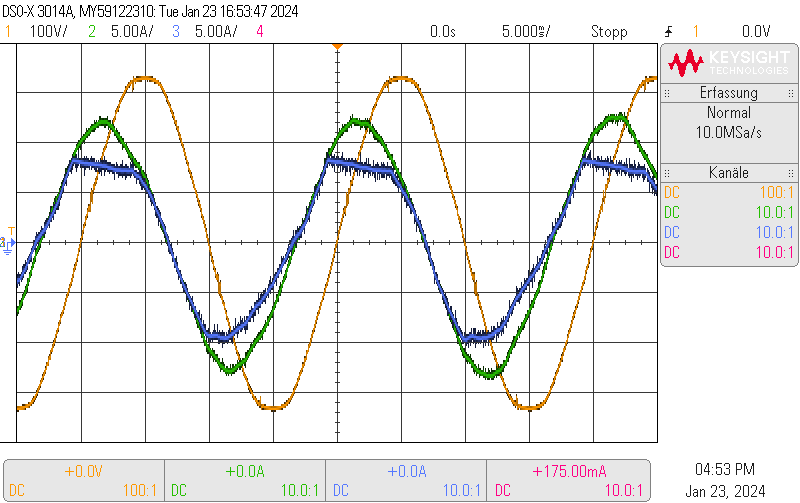
\includegraphics[width=0.8\textwidth]{./assets/images/3_5_1_ohneRotorstrom.png}
	\caption{Die Netz-Sternspannung und Netz-Leiterstrom bei einer Windgeschwindigkeit von 11m/s}
	\label{fig:oszi_dopp}
\end{figure}

\section{Auswertung}
\label{sec:auswertung}

Die drei Kurven $P_{el}(v_{\mathrm{wind}})$ für die direkte Netzkopplung, die Asynchronmaschine mit Umrichter und die doppeltgespeiste Asynchronmaschine sind in Abbildung~\ref{fig:auswertung_pel} zu sehen.

% FIXME: Bild fehlt
\begin{figure}[!ht]
  \centering

  \caption{Die Windgeschwindigkeit-Leistungs-Graphen für alle drei Anschlussarten in einem Plot}
  \label{fig:auswertung_pel}
\end{figure}

% TODO: Auswertung für das Bild schreiben und im Hinblick auf Kosten und Effizienz

Im Anschluss an die Messungen kann außerdem der Wirkungsgrad $\eta(v_{\mathrm{wind}}) = \frac{P_{\mathrm{el}}{P_{\mathrm{mech}}$ für jedes der Generatorsysteme erstellt werden. Alle drei Graphen in einem Plot sind in Abbildung~\ref{fig:auswertung_eta} dargestellt.

% FIXME: Bild fehlt
\begin{figure}[!ht]
	\centering

	\caption{Die Leistungs-Wirkungsgrad-Graphen für alle drei Generatorsysteme in einem Plot}
	\label{fig:auswertung_eta}
\end{figure}

% TODO: Ergebnis dieser Messung erläutern

Für das Verständis der doppelt gespeisten Asynchronmaschine werden nun die Ergebnisse aus der Messung nochmal genauer analysiert. Dafür werden die drei Funktionen $P_{el}(v_{\mathrm{wind}})$, $P_{R}(v_{\mathrm{wind}})$ und $P_{S}(v_{\mathrm{wind}})$ in einem Diagramm gemeinsam dargestellt.

% FIXME: Bild fehlt
\begin{figure}[!ht]
  \centering

  \caption{Die elektrische Leistung und die Ständer- und Rotorleistung in Abhängigkeit der Windgeschwindigkeit in einem Plot}
  \label{fig:auswertung_leistung}
\end{figure}

% TODO: Auswertung im Bezug auf die Theorie der doppelt gespeisten Asynchronmaschine schreiben

\section{Fazit}
\label{sec:fazit}

Dieses Praktikum hat deutlich gezeigt, wie wichtig die richtige Verschaltung der Windkraftanlage ist. Die Windkraftanlage mit direkter Netzkopplung ist zwar die einfachste Verschaltung, allerdings ist sie auch die ineffizienteste. Außerdem sind die Möglichkeiten zur Einstellungen eines Arbeitspunktes stark begrenzt. Die Windkraftanlage mit Vollumrichter bietet hier mehr Möglichkeiten und ist auch effizienter, ist im Aufbau allerdings auch teurer und komplizierter. Da die komplette Leistung über den Umrichter gesteuert wird, ist dieser natürlich groß auszulegen, wobei eigentlich nur in einem kleinen Drehzahlbereich eine Veränderung/Steuerung stattfindet. Ein doppelt gespeister Asynchronmotor vereint hier die Vorteile beider Schaltungen, da hier nur ein Bruchteil der Leistung tatsächlich über den Umrichter fließt. Dieser kann daher entsprechend kleiner ausgelegt werden. Allerdings sollte auch bedacht werden, dass für diese Schaltung mehr Aufwand von Nöten ist. Außerdem muss ein Transformator den Zwischenkreis speisen. Diese Auslegungsart lohnt sich nur für Windkraftanlagen ab $800$kW.



\end{document}
